\chapter{Auswertung der Ergebnisse}
Im Folgenden werden die unterschiedlichen Fahrstuhl-Scheduler miteinander verglichen. Dazu wurde eine Menge von Fahrstuhl-Rufen zusammengestellt, die im einfachen Scheduler zu einem nahezu konstanten Durchsatz f�hren. Dadurch, dass eine der Metriken konstant ist, sind die Unterschiede zwischen den Metriken der Scheduler deutlicher zu sehen.

F�r die Simulation wurde eine Zeitspanne von 200 Zeiteinheiten festgesetzt. Alle zwei Zeiteinheiten wird ein zuf�lliger Fahrstuhl-Ruf generiert, der vom Scheduler anschlie�end behandelt wird.

\section{Fahrstuhl ohne Wissen}
Im Folgenden werden die ermittelten Werte des einfachen Fahrstuhl-Schedulers dargestellt.

In Diagramm \ref{fig:notknowing_throughput} ist der Durchsatz des einfachen Schedulers dargestellt. Es ist zu sehen, dass der einfache Scheduler nach Ablauf der Simulationszeit 88 Fahrstuhl-Rufe erledigt hat.
\begin{figure}[H]
\centering
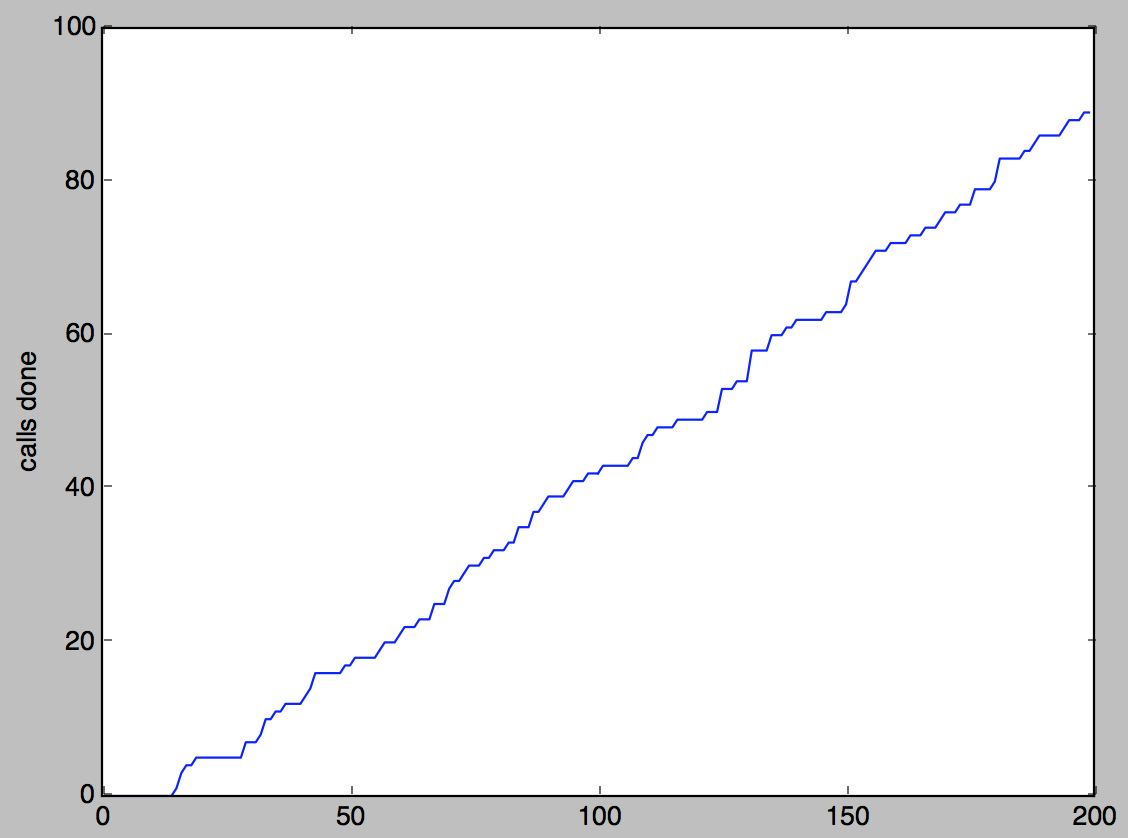
\includegraphics[width=0.5\linewidth]{./NotKnowing_Throughput}
\caption{Durchsatz des einfachen Schedulers}
\label{fig:notknowing_throughput}
\end{figure}

In Abbildung \ref{fig:notknowing_times} sind die durchschnittlichen Warte- und Fahrzeiten pro Zeiteinheit der Fahrstuhlrufe zu sehen.
\begin{figure}[htbp]
	\centering
	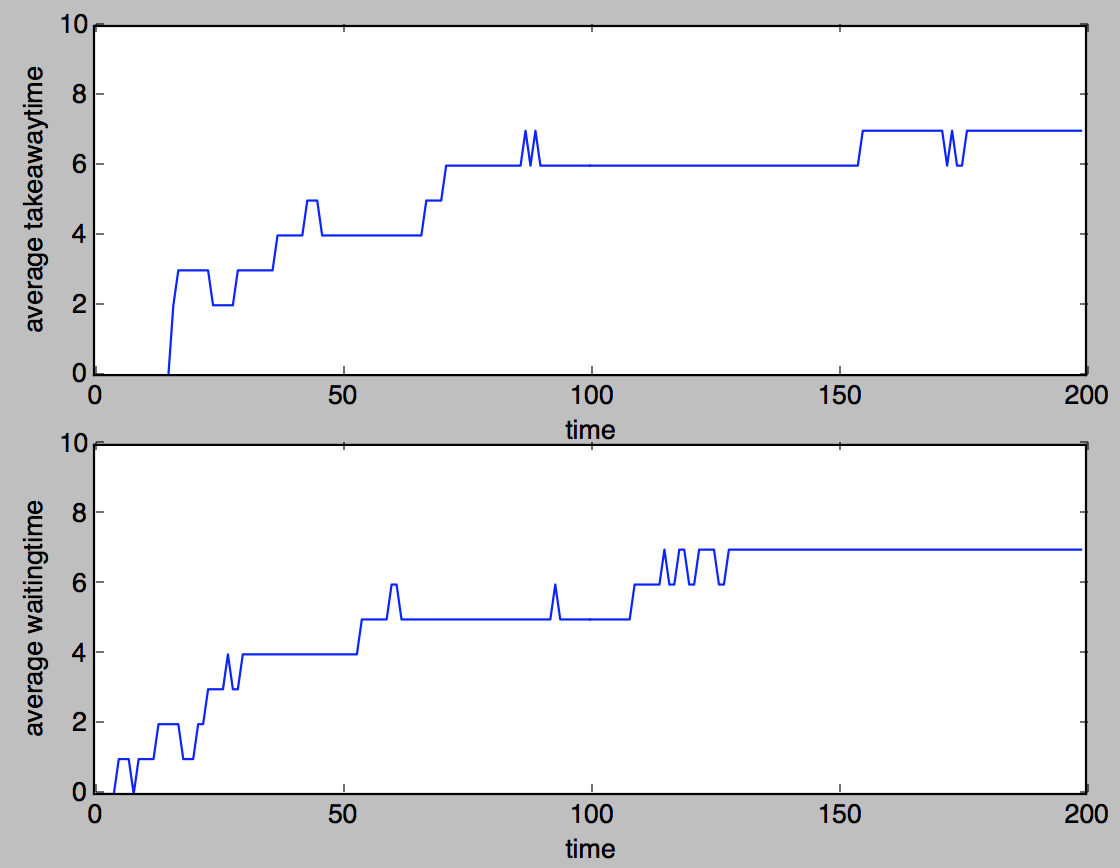
\includegraphics[width=0.7\linewidth]{./NotKnowing_Times}
	\caption{Zeiten des einfachen Schedulers}
	\label{fig:notknowing_times}
\end{figure}


\section{Fahrstuhl mit Wissen}
Im Folgenden werden die ermittelten Werte des wissenden Fahrstuhl-Schedulers dargestellt.

In Diagramm \ref{fig:knowing_throughput} ist der Durchsatz des einfachen Schedulers dargestellt. Es ist zu sehen, dass der wissende Scheduler nach Ablauf der Simulationszeit 92 Fahrstuhl-Rufe erledigt hat.
\begin{figure}[H]
	\centering
	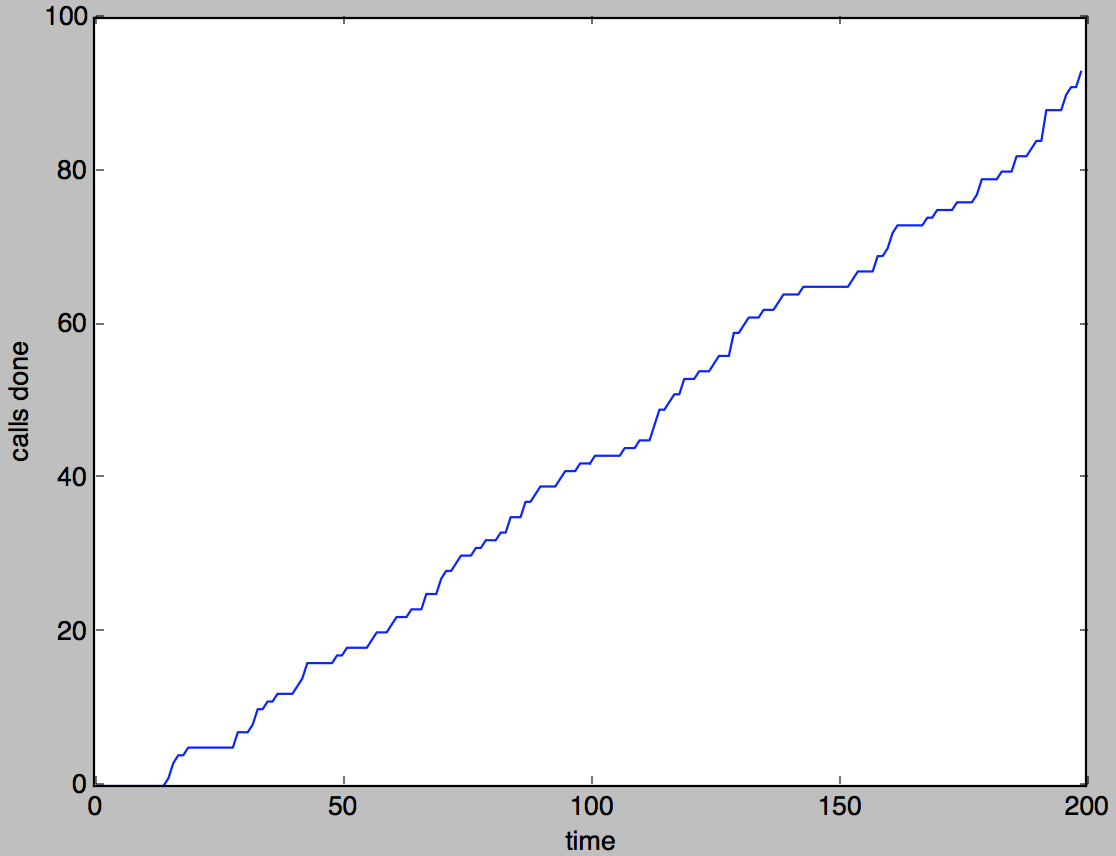
\includegraphics[width=0.5\linewidth]{./Knowing_Throughput}
	\caption{Durchsatz des wissenden Schedulers}
	\label{fig:knowing_throughput}
\end{figure}

In Abbildung \ref{fig:knowing_times} sind die durchschnittlichen Warte- und Fahrzeiten pro Zeiteinheit der Fahrstuhlrufe zu sehen.
\begin{figure}[htbp]
	\centering
	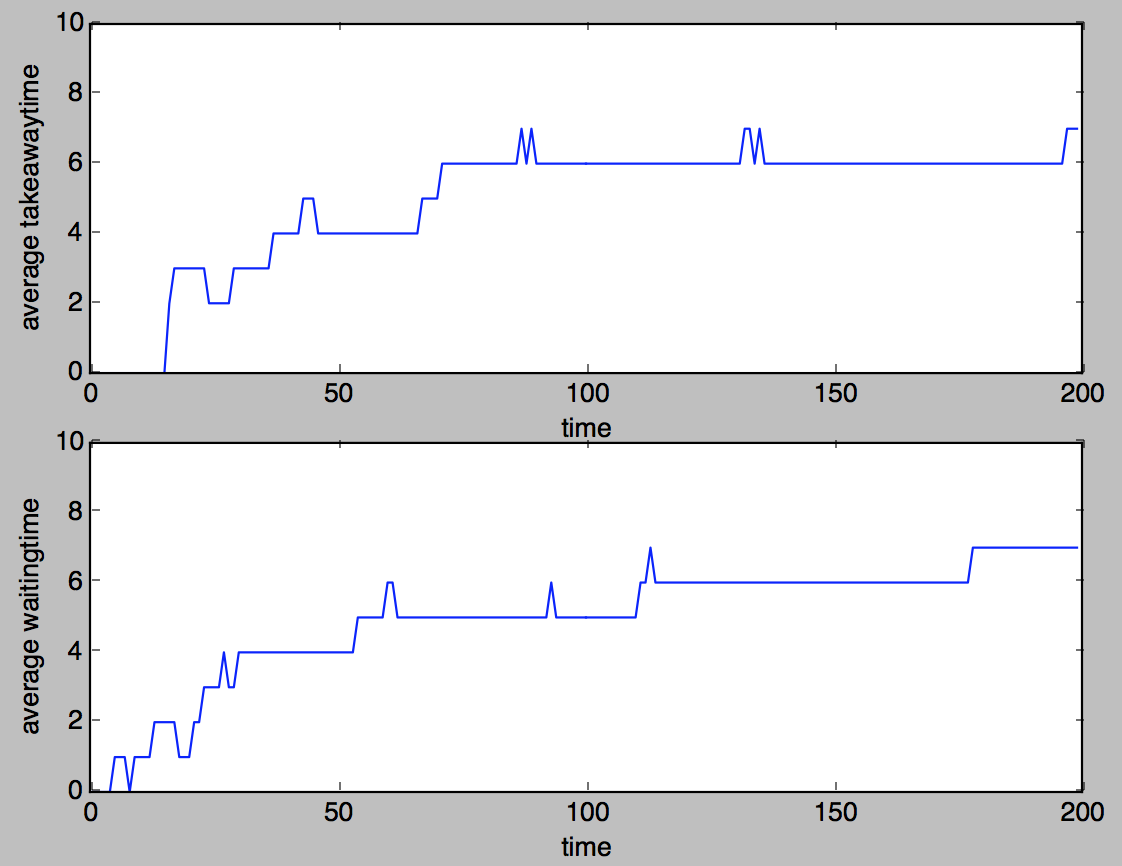
\includegraphics[width=0.7\linewidth]{./Knowing_Times}
	\caption{Zeiten des wissenden Schedulers}
	\label{fig:knowing_times}
\end{figure}

\section{Analyse}
Nimmt man die Abbildungen dieses Kapitels f�r sich, haben sie keine Aussagekraft. Im Folgenden werden sie miteinander verglichen, um einen Wert aus ihnen zu ziehen.

Vergleicht man die Durchsatz-Abbildungen, dann sieht man, dass der wissende Scheduler einige Fahrstuhlrufe mehr beendet hat als der einfache Scheduler. Dies ist auf die Konstellation der zuf�llig erstellen Fahrstuhlrufe zur�ckzuf�hren und ist f�r diese Betrachtung nicht von Interesse. Was au�erdem auff�llt ist, dass die Kurve anders verl�uft. Zum Zeitpunk 104 tritt der erste zuk�nftige Fahrstuhlruf auf. Man sieht in den Graphen, dass in der Kurve des wissenden Scheduler - im Vergleich zum einfachen Scheduler - an dieser Stelle weniger Rufe erledigt wurden. Dies liegt am ver�nderten Scheduling-Verhalten, das in in Abschnitt \ref{sec:model} erkl�rt wird. An den Zeitpunkten 118, 148 und 166 treten ebenfalls zuk�nftige Rufe auf. Zu diesen Zeitpunkten sind ebenfalls wieder niedriges Wachstum in Abbildung \ref{fig:knowing_throughput} zu finden.



